% Run: arara -l *.tex to generate a log file (arara.log) of the compilation for traceability and debugging.
% Running -l instead of -v is also quicker to run.

% synctex: on - an input and output synchronization feature that allows navigation from source to typeset material and vice versa.
% interaction: nonstopmode - Tex does not request input after serious errors but stops altogether.
% shell: yes - shell escape to add compilation parameters.

% arara: pdflatex: { synctex: on, interaction: nonstopmode, shell: yes }
% arara: pdflatex: { synctex: on, interaction: nonstopmode, shell: yes }


% hidelinks - removes the borders around clickable cross-references and hyperlinks

% draft - speeds up typesetting, because figures are not loaded, just indicated by a frame.
% Hyperref items will only be displayed without the functionality.
% The complication process using the "draft" option is quicker to run.
% Delete the "draft" option or replace it with "final" in the final document version.

\documentclass[conference]{IEEEtran}
\IEEEoverridecommandlockouts
% The preceding line is only needed to identify funding in the first footnote. If that is unneeded, please comment it out.
\usepackage{morewrites}
\usepackage[thicklines, makeroom]{cancel}
\usepackage{csvsimple}
\usepackage{siunitx}
\usepackage[bookmarks, bookmarksnumbered, bookmarksopen, breaklinks, pdftex, linktoc=all, pdfmenubar, hidelinks]{hyperref}
\usepackage{cite}
\usepackage{amsmath,amssymb,amsfonts}
\usepackage{algorithmic}
\usepackage{graphicx}
\usepackage{textcomp}
\usepackage{xcolor}
\usepackage{caption}
\usepackage{subcaption}
\usepackage{listings}
\usepackage{xurl}
\usepackage{enumitem}
\usepackage{tabto}
\usepackage{steinmetz}  % for having the phase angle
\usepackage{tikz}   % for plotting
\usepackage{pgfplots}   % for plotting
\usepgfplotslibrary{groupplots}
\hypersetup{pdftitle={ELEC 3909 Assignment \#1: Maxwell's Equations \& Waves in Lossy Media},
            pdfauthor={000000000 \& 000000000},
            pdfcreator={000000000}}

% A new command for less cramped nested fractions
\newcommand\ddfrac[2]{\frac{\displaystyle #1}{\displaystyle #2}}

% A path to the images directory to be imported in the tex document
\graphicspath{{./Imports/Images/}}


\def\BibTeX{{\rm B\kern-.05em{\sc i\kern-.025em b}\kern-.08em
    T\kern-.1667em\lower.7ex\hbox{E}\kern-.125emX}}
\begin{document}

\title{Plots examples in two columns setup\\
}

\author{\IEEEauthorblockN{student1 name \& student2 name
        \thanks{studentID, email: 000000000@cmail.carleton.ca}
        \thanks{studentID, email: 000000000@cmail.carleton.ca}
    }
}

\maketitle

% A single figure
\begin{figure}[htbp]
    \centering
    \includegraphics[width=0.65\linewidth]{q1-f1-v3.png}
    \caption{figure title}
    \label{fig:fig1Test}
\end{figure}



% two pictures in a sub-figure environment

% subfloat to specify that this is a sub-figure
% qquad means two squares
\begin{figure}[htbp]
    \centering
    \subfloat[\centering sub-figure 1 sub-title]{{\includegraphics[width=3.9cm]{q1-f1-v3.png} }}%
    \qquad
    \subfloat[\centering sub-figure 2 sub-title]{{\includegraphics[width=3.9cm]{q1-f2.png} }}%
    \caption{figure title}
    \label{fig:example}
\end{figure}


\begin{figure}[htbp]
    \centering
    \begin{tikzpicture}[yscale=0.7, xscale = 0.7]
        \begin{axis}[
                grid=both,
                ymin=0,
                ymax=1700,
                ylabel=E-field (V/m),
                %max space between ticks=1,
                xmin=0,
                xmax=150,
                xlabel=Distance (mm)]
            \addplot[color=red, style=thick]table[x=c, y=d, col sep=comma]{./Imports/Data/plot.csv};
        \end{axis}
    \end{tikzpicture}
    \caption{figure title}
    \label{fig:ee4}
\end{figure}



% Breaks to the second column
\pagebreak



% Two plots plotted using latex
\begin{figure}[htbp]
    \centering
    \subfloat[\centering sub-figure 1 sub-title]{{
        \begin{tikzpicture}[yscale=0.4, xscale=0.4]
        \begin{axis}[
                grid=both,
                ymin=-90,
                ymax=1,
                ylabel=dB,
                xmin=7,
                xmax=12,
                xlabel=Frequency (GHz)]
            \addplot[color=black, style=thick]table[x=a, y=b, col sep=comma]{./Imports/Data/q1sp.csv};
            \addplot[color=blue, style=thick]table[x=a, y=c, col sep=comma]{./Imports/Data/q1sp.csv};
            \addplot[color=red, style=thick]table[x=a, y=d, col sep=comma]{./Imports/Data/q1sp.csv};
            \addplot[color=green, style=thick]table[x=a, y=e, col sep=comma]{./Imports/Data/q1sp.csv};
            \legend{S(1\,1), S(2\,1), S(1\,2), S(2\,2)}
        \end{axis}
        \label{fig:1.1.1}
    \end{tikzpicture}
    }}%
    \qquad
    \subfloat[\centering sub-figure 2 sub-title]{{
        \begin{tikzpicture}[yscale=0.4, xscale=0.4]
            \begin{axis}[
                    grid=both,
                    ymin=-120,
                    ymax=1,
                    ylabel=dB,
                    %max space between ticks=1,
                    xmin=7,
                    xmax=12,
                    xlabel=Frequency (GHz)]
                \addplot[color=black, style=thick]table[x=a, y=b, col sep=comma]{./Imports/Data/q1sp2.csv};
                \addplot[color=blue, style=thick]table[x=a, y=c, col sep=comma]{./Imports/Data/q1sp2.csv};
                \addplot[color=red, style=thick]table[x=a, y=d, col sep=comma]{./Imports/Data/q1sp2.csv};
                \addplot[color=green, style=thick]table[x=a, y=e, col sep=comma]{./Imports/Data/q1sp2.csv};
                \legend{S(1\,1), S(2\,1), S(1\,2), S(2\,2)}
            \end{axis}
            \label{fig:1.1.2}
        \end{tikzpicture}
        }}%
    \caption{figure title}
    \label{fig:example5}
\end{figure}












\tikzset{every picture/.style={line width=0.75pt}} %set default line width to 0.75pt        

\begin{figure}[htbp]
\begin{center}
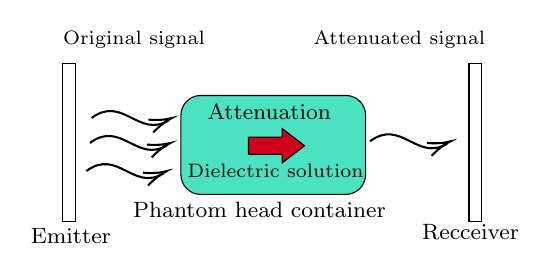
\begin{tikzpicture}[x=0.75pt,y=0.75pt,yscale=-1,xscale=1]
%uncomment if require: \path (0,300); %set diagram left start at 0, and has height of 300


\draw  [fill={rgb, 255:red, 74; green, 226; blue, 192 }  ,fill opacity=1 ] (103.96,61.04) .. controls (103.96,55.78) and (108.23,51.51) .. (113.5,51.51) -- (183.4,51.51) .. controls (188.66,51.51) and (192.93,55.78) .. (192.93,61.04) -- (192.93,89.65) .. controls (192.93,94.92) and (188.66,99.19) .. (183.4,99.19) -- (113.5,99.19) .. controls (108.23,99.19) and (103.96,94.92) .. (103.96,89.65) -- cycle ;
%Curve Lines [id:da5044457007963458] 
\draw [line width=0.75]    (60.93,62.36) .. controls (75.9,51.14) and (83.64,72.41) .. (98.1,63.46) ;
\draw [shift={(99.7,62.36)}, rotate = 159.24] [color={rgb, 255:red, 0; green, 0; blue, 0 }  ][line width=0.75]    (10.93,-3.29) .. controls (6.95,-1.4) and (3.31,-0.3) .. (0,0) .. controls (3.31,0.3) and (6.95,1.4) .. (10.93,3.29)   ;
%Curve Lines [id:da9697034123854519] 
\draw [line width=0.75]    (58.38,87.95) .. controls (73.35,76.72) and (81.09,97.99) .. (95.55,89.04) ;
\draw [shift={(97.15,87.95)}, rotate = 159.24] [color={rgb, 255:red, 0; green, 0; blue, 0 }  ][line width=0.75]    (10.93,-3.29) .. controls (6.95,-1.4) and (3.31,-0.3) .. (0,0) .. controls (3.31,0.3) and (6.95,1.4) .. (10.93,3.29)   ;
%Curve Lines [id:da60431380390168] 
\draw [line width=0.75]    (60.16,74.38) .. controls (75.12,63.16) and (82.87,84.42) .. (97.32,75.47) ;
\draw [shift={(98.93,74.38)}, rotate = 159.24] [color={rgb, 255:red, 0; green, 0; blue, 0 }  ][line width=0.75]    (10.93,-3.29) .. controls (6.95,-1.4) and (3.31,-0.3) .. (0,0) .. controls (3.31,0.3) and (6.95,1.4) .. (10.93,3.29)   ;
%Shape: Rectangle [id:dp4896020622971927] 
\draw   (46.98,36) -- (52.99,36) -- (52.99,112.37) -- (46.98,112.37) -- cycle ;
%Shape: Rectangle [id:dp8165874564737375] 
\draw   (242.75,36) -- (248.76,36) -- (248.76,112.37) -- (242.75,112.37) -- cycle ;
%Curve Lines [id:da8084381112436627] 
\draw [line width=0.75]    (195.07,73.6) .. controls (210.03,62.38) and (217.77,83.65) .. (232.23,74.7) ;
\draw [shift={(233.83,73.6)}, rotate = 159.24] [color={rgb, 255:red, 0; green, 0; blue, 0 }  ][line width=0.75]    (10.93,-3.29) .. controls (6.95,-1.4) and (3.31,-0.3) .. (0,0) .. controls (3.31,0.3) and (6.95,1.4) .. (10.93,3.29)   ;
%Right Arrow [id:dp4343437664934504] 
\draw  [fill={rgb, 255:red, 208; green, 2; blue, 27 }  ,fill opacity=1 ] (136.53,71.6) -- (152.71,71.6) -- (152.71,67.46) -- (163.5,75.73) -- (152.71,84) -- (152.71,79.87) -- (136.53,79.87) -- cycle ;

% Text Node
\draw (30.39,114.43) node [anchor=north west][inner sep=0.75pt]  [font=\footnotesize] [align=left] {Emitter};
% Text Node
\draw (45.93,19.16) node [anchor=north west][inner sep=0.75pt]  [font=\scriptsize] [align=left] {Original signal};
% Text Node
\draw (166.63,19.12) node [anchor=north west][inner sep=0.75pt]  [font=\scriptsize] [align=left] {Attenuated signal};
% Text Node
\draw (218.85,112.43) node [anchor=north west][inner sep=0.75pt]  [font=\footnotesize] [align=left] {Recceiver};
% Text Node
\draw (79.69,101.64) node [anchor=north west][inner sep=0.75pt]  [font=\footnotesize] [align=left] {Phantom head container};
% Text Node
\draw (105.91,83.13) node [anchor=north west][inner sep=0.75pt]  [font=\scriptsize] [align=left] {Dielectric solution};
% Text Node
\draw (115.5,54.51) node [anchor=north west][inner sep=0.75pt]  [font=\footnotesize] [align=left] {Attenuation};


\end{tikzpicture}
\caption{tikzPic}
\label{fig:3problem}
\end{center}
\end{figure}








\end{document}
